\documentclass[a4paper,10pt,egregdoesnotlikesansseriftitles]{scrartcl}
%\documentclass[a4paper,11pt]{report}

\usepackage[utf8]{inputenc}
%\usepackage[T1]{fontenc}
%\usepackage[toc,page]{appendix}

%remove helvetica/arial if necessary
%\usepackage[scaled]{helvet}
%\usepackage[default,regular,bold]{sourceserifpro}

\renewcommand\familydefault{lmr}
\usepackage{lmodern}
\usepackage{inconsolata}

\usepackage[pdfusetitle,hidelinks]{hyperref}
\usepackage{url}
\usepackage[dvipsnames]{xcolor}
\usepackage[inline]{enumitem}
\usepackage[final]{pdfpages}
\usepackage{graphicx}
\graphicspath{{figures/}}
\usepackage{wrapfig}
\usepackage{tabularx}
\usepackage[font=small,bf,normal]{caption}
\usepackage{subcaption}
\usepackage{tikz,pgfplots}
\pgfplotsset{compat=1.9}
\usetikzlibrary{arrows,automata,positioning,backgrounds,chains}

\usepackage{csquotes}
\usepackage{ragged2e}
\usepackage{mathtools}
\usepackage[many]{tcolorbox}
\usepackage[official]{eurosym}
\usepackage[hang,flushmargin]{footmisc}
\usepackage[colorinlistoftodos,prependcaption,textsize=scriptsize]{todonotes}

\newcommand{\fillin}[1]{\todo[inline,color=red!40,size=]{#1}}

\usepackage[capitalize]{cleveref}

%reduce margins
\usepackage{geometry}
%\geometry{textheight=680pt}
% \geometry{textheight=680pt,
%           top=2cm,
%           right=2cm,
%           left=2cm,
%           bottom=2.5cm,
%           marginparwidth=40pt,
%           footskip=15pt
%           }

% \RedeclareSectionCommand[
%   beforeskip=-\baselineskip,
%   afterskip=.35\baselineskip]{section}
% \RedeclareSectionCommand[
%   beforeskip=-.75\baselineskip,
%   afterskip=.4\baselineskip]{subsection}
% \RedeclareSectionCommand[
%   beforeskip=-.5\baselineskip,
%   afterskip=.2\baselineskip]{subsubsection}
% \RedeclareSectionCommand[
%   beforeskip=.5\baselineskip,
%   afterskip=-1em]{paragraph}
% \RedeclareSectionCommand[
%   beforeskip=-.5\baselineskip,
%   afterskip=-1em]{subparagraph}

%TODO remove
%\usepackage{showframe}

\newlist{compactitem}{itemize}{3}
\setlist[compactitem]{topsep=0pt,partopsep=0pt,itemsep=0pt,parsep=0pt}
\setlist[compactitem,1]{label=\textbullet}
\setlist[compactitem,2]{label=---}
\setlist[compactitem,3]{label=*}

%reduce author size in titlepage
%\usepackage[affil-it]{authblk} 
%\renewcommand\Authfont{\fontsize{11}{12}\selectfont}
%\renewcommand\Affilfont{\fontsize{9}{10.8}\itshape}
%\renewcommand*{\Authsep}{, }
%\renewcommand*{\Authand}{, }
%\renewcommand*{\Authands}{, }

\usepackage{etoolbox}
%\patchcmd{\maketitle}{\LARGE \@title}{\fontsize{16}{19.2}selectfont\@title}{}{}

\usepackage{listings}
\crefname{lstlisting}{listing}{listings}
\Crefname{lstlisting}{Listing}{Listings}
\lstset{basicstyle=\scriptsize,
        backgroundcolor=\color{lightgray},
        % xleftmargin=1em,
        % xtopmargin=1em,
        % xrightmargin=1em,
        % xbottommargin=1em,
        frame=tlbr,framesep=2pt,framerule=0pt
}
\lstset{language=C++,
      basicstyle=\scriptsize\ttfamily,
      keywordstyle=\color{blue}\ttfamily,
      stringstyle=\color{red}\ttfamily,
      commentstyle=\color{green}\ttfamily,
      morecomment=[l][\color{magenta}]{\#}
}

\usepackage{protobuf/lang}  % include language definition for protobuf

\usepackage[
        bibstyle=ieee,
        citestyle=numeric-comp,
        backend=biber,
        bibencoding=auto,
        %defernumbers=true,
        %url=false
        ]{biblatex}

\bibliography{proj_docu.bib}

\renewcommand*{\bibfont}{\footnotesize}
\renewcommand\mkbibacro[1]{{\footnotesize\MakeUppercase{#1}}}
%\renewcommand\mkbibacro[1]{{\MakeUppercase{#1}}}

\AtEveryBibitem{%
  %\ifentrytype{misc}{%
  %  \clearfield{url}%
  %  \clearfield{urldate}%
  %}%
  \ifentrytype{article}{%
    \clearfield{url}%
    \clearfield{urldate}%
    \clearfield{urlyear}%
  }{}%
  \ifentrytype{book}{%
    \clearfield{url}%
    \clearfield{urldate}%
    \clearfield{urlyear}%
  }{}%
  \ifentrytype{incollection}{%
    \clearfield{url}%
    \clearfield{urldate}%
    \clearfield{urlyear}%
  }{}%
  \ifentrytype{inproceedings}{%
    \clearfield{url}%
    \clearfield{urldate}%
    \clearfield{urlyear}%
  }{}%
  \ifentrytype{report}{%
    \clearfield{url}%
    \clearfield{urldate}%
    \clearfield{urlyear}%
  }{}%
  \ifentrytype{techreport}{%
    \clearfield{url}%
    \clearfield{urldate}%
    \clearfield{urlyear}%
  }{}%
  \iffieldundef{doi}{}{%
    \clearfield{issn}%
    \clearfield{isbn}%
  }%
}

\makeatletter
\defbibenvironment{bibliography}
{\list{\printtext[labelnumberwidth]{%
    \printfield{prefixnumber}%
    \printfield{labelnumber}}}
{%
\setlength{\bibhang}{0pt}%
\setlength{\leftmargin}{0pt}%
%\setlength{\leftmargin}{2em}%
\setlength{\itemindent}{2em}%
\setlength{\itemsep}{\bibitemsep}%
\setlength{\parsep}{\bibparsep}%
}}
{\endlist}
{\item}
\makeatother

\usepackage{setspace}
%use 1.5 line spacing
\onehalfspacing

%reduce margins and move title upwards, save trees! :)
%\usepackage[margin=0.8in]{geometry}
%\usepackage{titling}
% \setlength{\droptitle}{-8em}
% \pretitle{\begin{center}\fontsize{20pt}{20pt}\selectfont}
% \posttitle{\par\end{center}}
%\preauthor{\begin{center}\fontsize{14bp}{14bp}\selectfont}
%    \postauthor{\par\end{center}\vspace{24bp}}
% \predate{}
% \date{}
% \postdate{}

\newcommand{\review}[1]{{%
  \color{red}{#1}%
  }}

\urlstyle{same}

\usepackage[toc,acronyms,nogroupskip]{glossaries}
\setglossarystyle{list}
\renewcommand*{\glsgroupskip}{}
% first use of glossaryentry will be italic
\defglsentryfmt[main]{%
  \ifglsused{\glslabel}{%
    \glsgenentryfmt%
  }{%
    % Typeset first use
    \textit{\glsgenentryfmt}%
  }%
}

\makeglossaries
%!TEX root = ../proj_docu.tex

\newacronym{mc}{MCU}{MicroController Unit}
\newacronym{rf}{RF}{Radio Frequency}
\newacronym{iot}{I{o}{T}}{Internet of Things}
%\newacronym{qos}{QoS}{Quality of Service}
\newacronym{rdc}{RDC}{Radio Duty Cycling}
\newacronym{ap}{AP}{Access Point}
\newacronym{tls}{TLS}{Transport Layer Security}
\newacronym{hmac}{HMAC}{keyed-Hash Message Authentication Code}
\newacronym{sha}{SHA}{Secure Hash Algorithms}

\newglossaryentry{mqtt}
{
  name=MQTT,
  description={MQTT is a machine-to-machine (M2M)/"Internet of Things" connectivity protocol. It was designed as an extremely lightweight publish/subscribe messaging transport.}
}
%\glsdisablehyper

\glsaddall

\title{Project Documentation}
\subtitle{182.753 Internet of Things (VU 4,0) 2017W}

\newtcolorbox{sumbox}[2][]{
  colback=white,
  arc=0.5mm,
  colbacktitle=gray!5!white,coltitle=black,
  boxrule=1px,
  fonttitle=\bfseries\small,
  fontupper=\footnotesize,
  title={#2},
  #1
  }

\author{\texorpdfstring{%
  Philipp Raich\thanks{~\href{mailto:philipp.raich@tuwien.ac.at}{philipp.raich@tuwien.ac.at}} \and
  Mino Sharkhawy\thanks{~\href{mailto:mino.sharkhawy@student.tuwien.ac.at}{mino.sharkhawy@student.tuwien.ac.at}} \and
  Thomas Weber\thanks{~\href{mailto:thomas.weber@student.tuwien.ac.at}{e1025654@student.tuwien.ac.at}}
  }%
  {Philipp Raich, Mino Sharkhawy, Thomas Weber}%
}

\hypersetup{
  unicode=true,
  %pdfauthor={Philipp Raich},
  pdfsubject={Lab protocol},
  pdfkeywords={IoT, MQTT, ESP8266, LP-RF},
  pdfpagemode={UseOutlines},
}

\pagenumbering{alph}
\begin{document}

\begin{singlespacing}
\maketitle
%%!TEX root = ../proj_docu.tex

\makeatletter
\begin{titlepage}


\vspace{4cm}
\begin{minipage}{0.5\linewidth}
	%\includegraphics[height=47pt]{figures/asg-logo.pdf}
\end{minipage}
\begin{minipage}{0.45\linewidth}
\begin{flushright}
	\begin{minipage}{0.6\linewidth}
		\begin{flushright}
		% \begin{singlespace}
		% 	{\scriptsize Technische Universität Wien\\
		% 		Prof. Dr. Sabine Seidler (Rektor)\\
		% 		Karlsplatz 13\\
		% 		1040 Vienna\\}
		% \end{singlespace}
		\end{flushright}
	\end{minipage}
	\hspace{2pt}
	\begin{minipage}{0.23\linewidth}
		\begin{flushright}
		
\includegraphics[height=50pt]{figures/TU_Signet}
		\end{flushright}
	\end{minipage}
\end{flushright}
\end{minipage}

\vspace{4cm}
\begin{center}
{\Large \@subtitle}\\
%\vspace{1cm}
%{\huge \textbf{IoT WS17/18}}\\
\vspace{1.5em}
{\huge \textbf{\@title}}
\vspace{4cm}
\end{center}


%\vfill

\begin{singlespace}
\begin{tabular}{l l}
	\@author
\end{tabular}
\end{singlespace}

%\thispagestyle{empty}
%\pagestyle{empty}

\end{titlepage}
\makeatother

%\pagenumbering{alph} % set the numbering style to lowercase letter
\setcounter{tocdepth}{2}

\tableofcontents
\end{singlespacing}

\thispagestyle{empty}

%!TEX root = ../proj_docu.tex

\pagenumbering{arabic} % set the numbering style to arabic
\setcounter{page}{1} % Set the page counter to 1

\section{Introduction}

This document serves as documentation and lab protocol for the lab part of the \textit{Internet of Things} course at TU Vienna (WS2017). It contains the given assignment, details about the given tasks and questions, and finally a description of the team's submitted work.


\section{Assignment}
\label{sec:assignment}

The context of the assignment was given as: Multiple low-power \textbf{sensor nodes}/\glspl{mc} shall be connected to a special purpose, \textbf{WiFi-enabled \gls{mc}} using a generic \gls{rf}-module. The WiFi-enabled \gls{mc} will act as a \textbf{gateway} for the sensor nodes, i.e. it is intended to deliver or save the sensor readings and serve them over WiFi either
\begin{enumerate*}[label=(\alph*)]
  \item as \textbf{\gls{mqtt} client} to a broker, and thus consumers/subscribers, or
  \item as a web server, serving a \textbf{homepage} with sensor charts over HTTP
\end{enumerate*}.

Further, the \gls{rf} protocol used between the sensor nodes and the gateway device must focus on \textbf{low energy consumption}, to extend the battery life of the sensor nodes, through e.g. \gls{rdc} and similar measures. The gateway device will be connected to an outlet and does not have to hold up to the same scrutiny. The sensor-nodes and the gateway device to be used will be supplied. The project work consist of writing the necessary software and evaluating the end result.

The \gls{rf}-modules to be used for the low power radio communication (LP-RF) are based on the 2.4GHz \textbf{nRF24L01+}\footnote{\url{http://www.nordicsemi.com/eng/Products/2.4GHz-RF/nRF24LU1P}}, which implements the proprietary ``Enhanced ShockBurst'' protocol. The sensor-nodes are compatible to ``Arduino Pro Mini 3.3V'' (ATmega328P@MHz) devices\footnote{\url{https://store.arduino.cc/arduino-pro-mini}}.

The given cornerstones and deliverables were determined as following:

\begin{sumbox}{Cornerstones}
\begin{compactitem}
  \item Design a communication protocol based on the nRF24L01+ ``Enhanced SchockBurst'' protocol. Consider the energy consumption and limit it to a possible minimum (battery powered sensor nodes).
  \item Make the sensor data available to the ``home network'', i.e. to conventional OTS hardware, via WiFi or Ethernet (via gateway device).
  \item The data should be protected from access by third parties, even if they have access to the home network (authenticated access).
\end{compactitem}
\end{sumbox}

For the sake of focus on the main scope of the project, the following simplifications apply:
\begin{enumerate*}[label=(\alph*)]
  \item The sensor readings can be ``simulated''/mocked, and
  \item security considerations regarding the low-power \gls{rf}-protocol can be widely ignored
\end{enumerate*}.

\begin{sumbox}{Deliverables}
\begin{compactitem}
  \item All the written \textbf{code}.
  \item A \textbf{presentation} of the completed project shall be given.
  \item A clean \textbf{documentation} and \textbf{lab-protocol} must be submitted (this file). The documentation shall complete the submitted code and explain how the tasks were solved.
\end{compactitem}
\end{sumbox}


\section{Solution}

\subsection{Architecture}

We chose to follow variant \textit{(a)} of the assignment, i.e. to map the messages from the sensor-nodes to \gls{mqtt} on the gateway node (see~\cref{fig:arch_overview}). Additionally, a dedicated device (BeagleBone Black Industrial\footnote{\url{https://beagleboard.org/arrowbbbi}}) was employed to cover the following tasks:
\begin{enumerate*}[label=(\alph*)]
  \item act as a \textbf{WiFi \gls{ap}} (and DHCP),
  \item run a \textbf{\gls{mqtt} broker}, and
  \item serve as clock source.
\end{enumerate*}
\textit{hostapd} and \textit{dnsmasq} were used to serve the \gls{ap} functionality, while \textit{mosquitto} was used as a \gls{mqtt} v3.1/v3.1.1 compliant \gls{mqtt} broker.

\begin{figure}[htb]
  \centering
  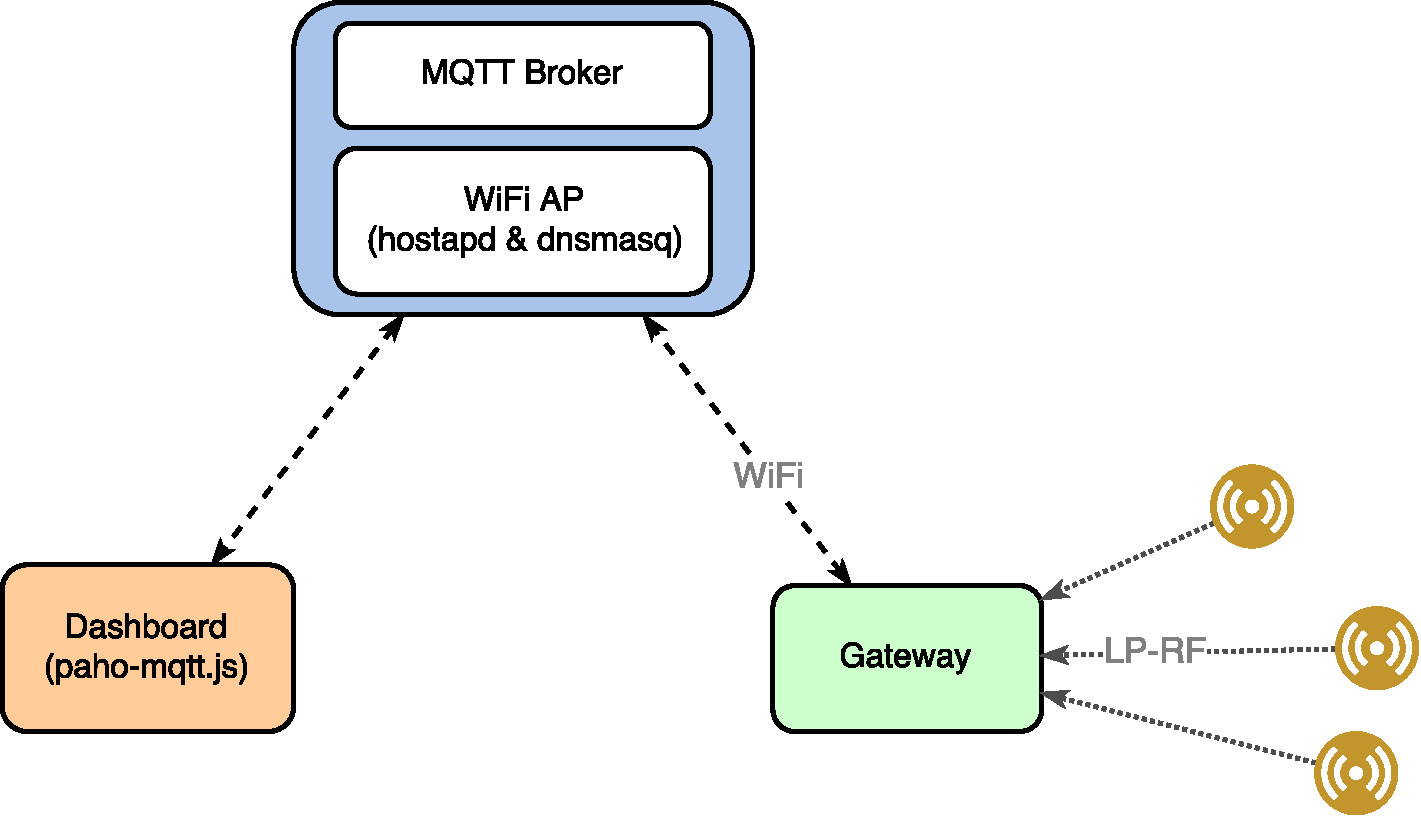
\includegraphics[width=0.55\linewidth]{arch_overview.pdf}
  \caption{Overview over the chosen architecture.}
  \label{fig:arch_overview}
\end{figure}

Diverging from the task description, a HTML \textbf{dashboard} was developed \emph{additionally} to the \gls{mqtt} broker, which would receive the data from the \gls{mqtt} broker via a JavaScript \gls{mqtt} client (over websockets).

This architecture of loosely coupled components allows for a robust implementation that avoids interferences between components, which are a common threat on \gls{iot} solutions that employ ``jack-of-all-trades'' components. Further, established libraries and packages are available, and the team can concentrate on the main tasks of the project. Moving as much as logic as possible from particularly the underpowered gateway was considered a main priority.


\subsection{Security}
\label{sec:security}

The following security threats were identified:

\begin{compactitem}
  \item eavesdropping (confidentiality),
  \item data manipulation/message forgery (authenticity).
\end{compactitem}

To protect the \gls{mqtt} messages/connections against these threats, \textbf{\gls{tls} with client certificates} were used, to authenticate the participating endpoints and protect the transmitted data. Additionally, \textbf{user-name and password authentication} was used for \gls{mqtt} client authentication with the broker (see \gls{mqtt} configuration in~\cref{sec:broker}).

To protect the LP-RF protocol between nodes and gateway, \gls{hmac} with timestamped messages was used (see~\cref{sec:hmac}), using pre-shared keys deployed at programming. The timestamped messages allow for detection of replay attacks, since old/repeated messages can be discarded. Please note that \gls{hmac} will not protect against eavesdropping.


\subsection{Parts}

The parts of the solution thus are:

\begin{compactitem}
  \item A low-power \gls{rf} protocol for communication between sensors and gateway (\cref{sec:rf_proto})
  \item Sensor node program (\cref{sec:sens_node})
  \item Gateway program, with \gls{mqtt} topic mapping (\cref{sec:gateway})
  \item A \gls{mqtt} broker and respective configuration (\cref{sec:broker})
  \item A HTTP Dashboard (\cref{sec:dashboard})
\end{compactitem}


\subsubsection{Low Power RF Protocol}
\label{sec:rf_proto}

A enhanced library around the ``Enhanced ShockBurst''-API was designed, specific to the requirements of the given task. The public functions of the API are listed in~\cref{lst:rf_api}.

\begin{lstlisting}[language=C++,label=lst:rf_api,caption="RF Wrapper Library API"]
int rflib_sensor_init(uint16_t cepin, uint16_t cspin, uint8_t channel,
          uint64_t address, uint8_t delay, uint8_t retransmits);
void rflib_sensor_tx_pre(void);
int rflib_sensor_tx(const struct rflib_msg_t *msg, struct rflib_msg_t *ackmsg);
void rflib_sensor_tx_post(void);

int rflib_coordinator_init(uint16_t cepin, uint16_t cspin, uint8_t channel,
         const uint64_t *addresses, uint8_t n_addresses,
         uint8_t delay, uint8_t retransmits);
int rflib_coordinator_available(void);
void rflib_coordinator_read(struct rflib_msg_t *msg);
int rflib_coordinator_set_reply(uint8_t address_idx, struct rflib_msg_t *msg);
void rflib_coordinator_clear_reply(void);
\end{lstlisting}

The API is split into \textit{sensor} and \textit{coordinator} specific functions, to accommodate the distinction between highly constrained sensor nodes and the ``unconstrained'' gateway device, which acts as coordinator. The sensor-specific interface thus includes the \lstinline{rflib_sensor_tx_pre()} and \lstinline{rflib_sensor_tx_post()} functions, that allow the sensor to execute specific actions before and after sending data. In particular, the RF-chip on sensor nodes is \textbf{disabled} between sending messages, as are all unnecessary parts of the system, e.g. any connected sensors, and the attached RTC-chip is set to wake the system at the latest configurable time, or when the next sensor message is due, whichever comes earlier. This allows to reduce the power consumption to a minimum.


\paragraph{Message Authentication}
\label{sec:hmac}

\Gls{hmac} was employed to authenticate and verify the integrity of individual messages, using the \gls{sha}-1 function (\gls{hmac}-\gls{sha}-1) with pre-shared keys. The keys are deployed on the nodes during programming. This protects the messages sent over the LP-RF network against message forging. Replay attacks are averted by including a timestamp in the message (see~\cref{lst:msg_format,sec:msg_sequence}).


\paragraph{Energy Considerations}
Special care had to be taken to avoid unnecessary energy consumption by the \gls{rf}-module on the sensor nodes, which together with the peculiarities of the ``Enhanced ShockBurst''-protocol lead to the following measures:

\begin{compactitem}
  \item The \gls{rf}-module on the sensor nodes was \textbf{disabled whenever possible}, and only enabled for data transmissions.
  \item Sensors were disabled/shut-off when not needed, and only enabled when actively taking measurements.
  \item Data can still be received by the sensor nodes by ``piggybacking'' on ACKs (i.e. in response to packets from the sensor) (cf.~\cref{sec:msg_sequence}).
  \item The interval at which the sensor nodes wake up for transmissions is configurable.
\end{compactitem}


\paragraph{Message and Data Format}
\label{sec:msg_format}

Protocol Buffers\footnote{\url{https://developers.google.com/protocol-buffers/docs/proto}} were used to format the messages across RF nodes and gate. \cref{lst:msg_format} shows the corresponding structure.

\begin{lstlisting}[language=protobuf2,label=lst:msg_format,caption="Message Format as Protocol Buffer definition"]
message Command {
  enum CommandType {
    NEW_UPDATE_INTERVAL = 1;
  }
  required CommandType type = 1;
  optional sfixed32 param1 = 2;
  optional sfixed32 param2 = 3;
  optional sfixed32 param3 = 4;
}

message N2C {
  required fixed32 timestamp = 1;
  required fixed32 roomNo = 2;
  required uint32 nodeId = 3;
  required uint32 sensorId = 4;
  enum SensorType {
    TEMPERATURE = 1;
    HUMIDITY = 2;
  }
  required SensorType type = 5;
  required float data = 6;
}

message C2N {
  required fixed32 timestamp = 1;
  optional Command command = 2;
}
\end{lstlisting}

2 different types of messages are possible, \lstinline{N2C} for node to coordinator messages (sensor values) and \lstinline{C2N} for messages from coordinator to the nodes, which will are appended to the ACKs to the nodes on reception of a message from the nodes. The messages from coordinator to the nodes can \emph{additionally} contain a new update interval, to set the sensor sending frequency of the nodes.


\paragraph{Messaging Sequence}
\label{sec:msg_sequence}

To counteract replay attacks (cf.~\cref{sec:security}), messages from the coordinator contain a \textbf{timestamp} and are rejected by the nodes if the timestamp is \emph{not} newer than the last known timestamp. The coordinator on the other hand will reject messages that contain a timestamp outside of the update interval of the sensors. Since this requires the nodes and coordinator to agree on a common (although not necessarily perfectly accurate) time, it is required that the coordinator
\begin{itemize*}
  \item has a monotonous clock source, and
  \item ``broadcasts'' timestamps to the sensor nodes.
\end{itemize*}

The clock source is constructed by regularly publishing \emph{a} current time to the \gls{mqtt} topic
\begin{lstlisting}
  IoT/Time
\end{lstlisting}
which the coordinator is subscribed to, in order to update its own time and to send the nodes time updates (via the respective ACKs).

\paragraph{Known Issues}

\begin{compactitem}
  \item \Gls{hmac} will only guard the LP-RF protocol against forgery, and together with timestamps against replay attacks, but not against eavesdropping. This was accepted, since \gls{hmac} already exceeds the assignment specification, and encryption was not a requirement.
\end{compactitem}

\subsubsection{Sensor Node}
\label{sec:sens_node}

The sensor nodes were designed to deliver sensor data (at a configurable frequency) to the coordinator, using the protocol depicted in \cref{sec:rf_proto}.

For the data to be submitted, sensor mockups (generated data) were used to simulate actual sensors connected to the sensor nodes.

As a proof of concept, an available moisture sensor was connected to the sensor board. The pinout is shown in \Cref{fig:sensor_pinout}.

\begin{figure}[htb]
  \centering
  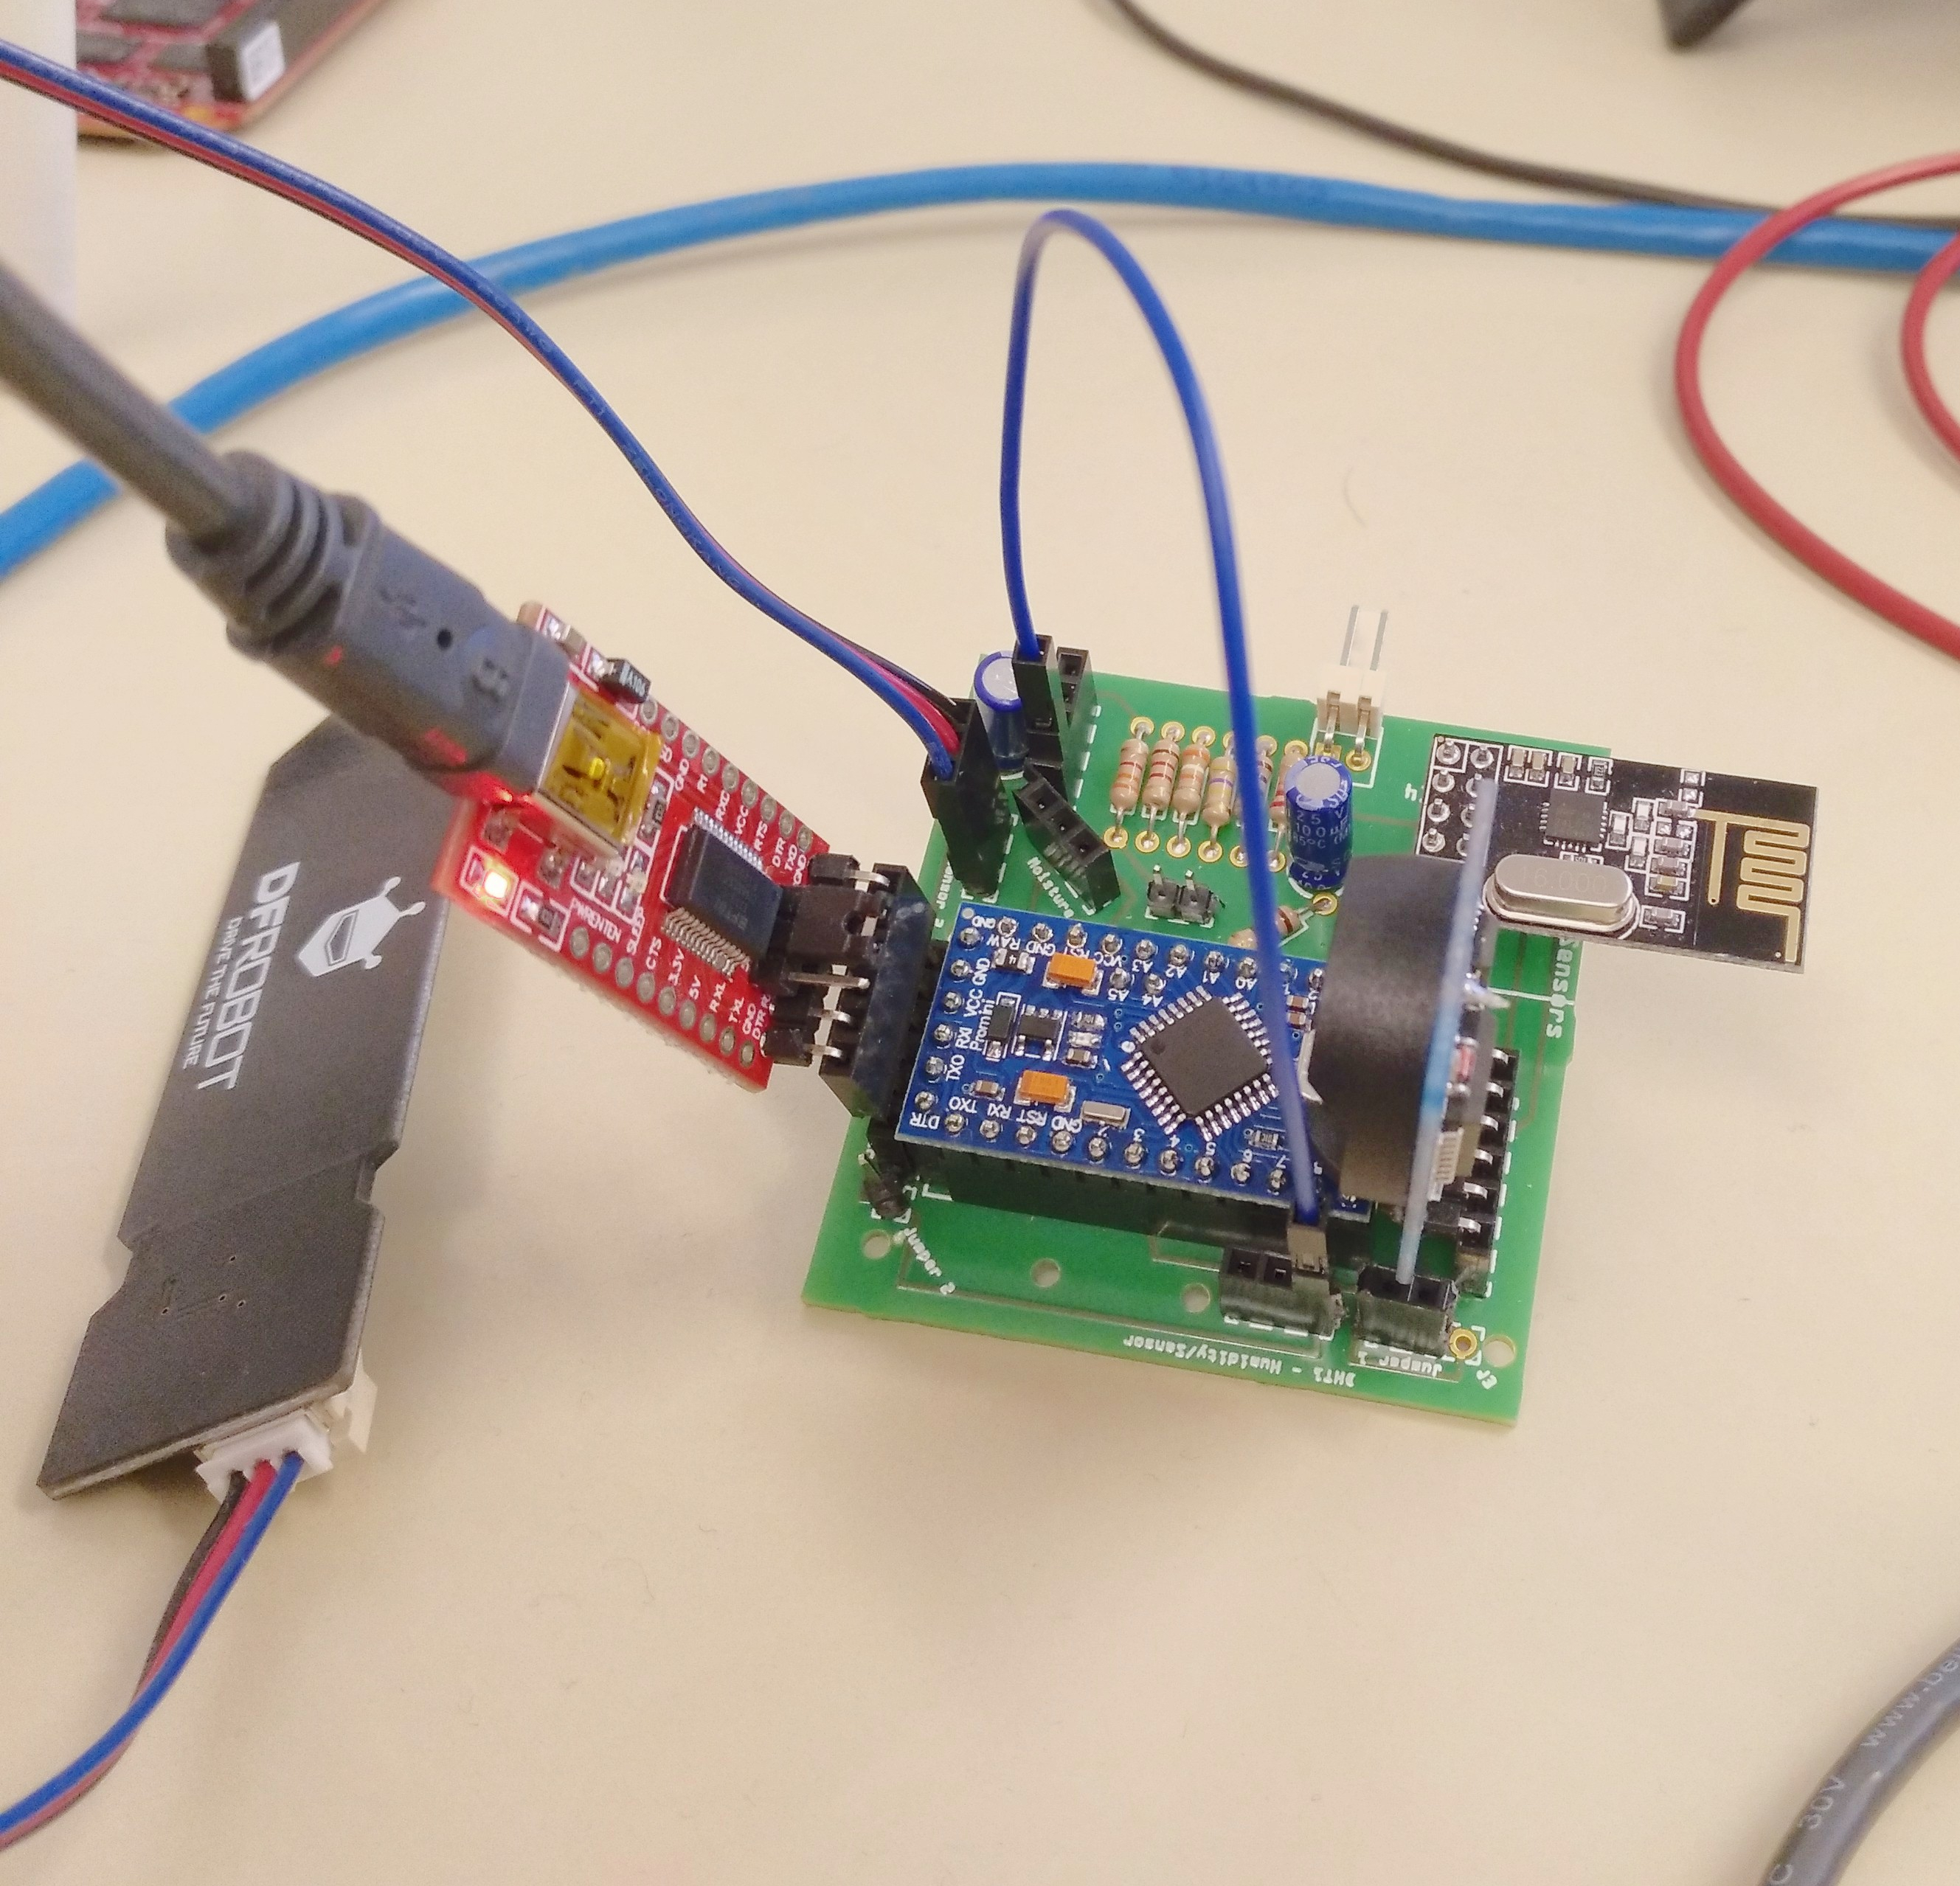
\includegraphics[width=0.25\linewidth]{pinout_moisture.jpg}
  \caption{PoC: Moisture Sensor Pinout}
  \label{fig:sensor_pinout}
\end{figure}

\paragraph{Configuration}

\begin{lstlisting}[language=C++,label=lst:node_config,caption="Config struct for the Nodes"]
struct rfnode_config cfg_node1 = {
  /* operations */
  .sensors = sensors_node1,
  .room_number = 1,
  .node_id = 1,
  .wakeup_interval = 30,
  /* communications */
  .address = 0xF0F0F0F0E1LL,
  .channel = 0,
  .delay = 15,
  .retransmits = 15,
  /* security */
  .auth_key = { 0x00, 0x00, 0x00, 0x00, 0x00, 0x00, 0x00, 0x00, 0x00, 0x00, 0x00, 0x00, 0x00, 0x00, 0x00, 0x00 },
  /* hardware */
  .cepin = 9,
  .cspin = 10,
  .rtcpin = 2,
  .rtcint = 0,
  /* debug */
  .baud_rate = 57600,
  .debug = DEBUG_ALL,
};
\end{lstlisting}


\subsubsection{Gateway}
\label{sec:gateway}

The main goals of the gateway device are:
\begin{compactitem}
  \item Act as a \textbf{border router} between the two distinct networks\footnote{With reduced capabilities as a non-transparent gateway, since it acts as a proxy and bridges merely on the application-layer.}.
  \item Act as the \textbf{coordinator} for the sensor network.
  \item Map between sensors nodes (respectively their sensors) and \gls{mqtt} topics.
  \item Relay control commands to the sensor nodes.
\end{compactitem}

For the communication with the sensor network, the gateway thus is equipped with the same \gls{rf}-module (nRF24L01+) as the sensor nodes, and uses the \gls{rf}-wrappers from \cref{sec:rf_proto}, although the coordinator-specific functions. For this purpose, the pinout shown in \cref{fig:pinout_coordinator} was used.

\begin{figure}[htb]
  \centering
  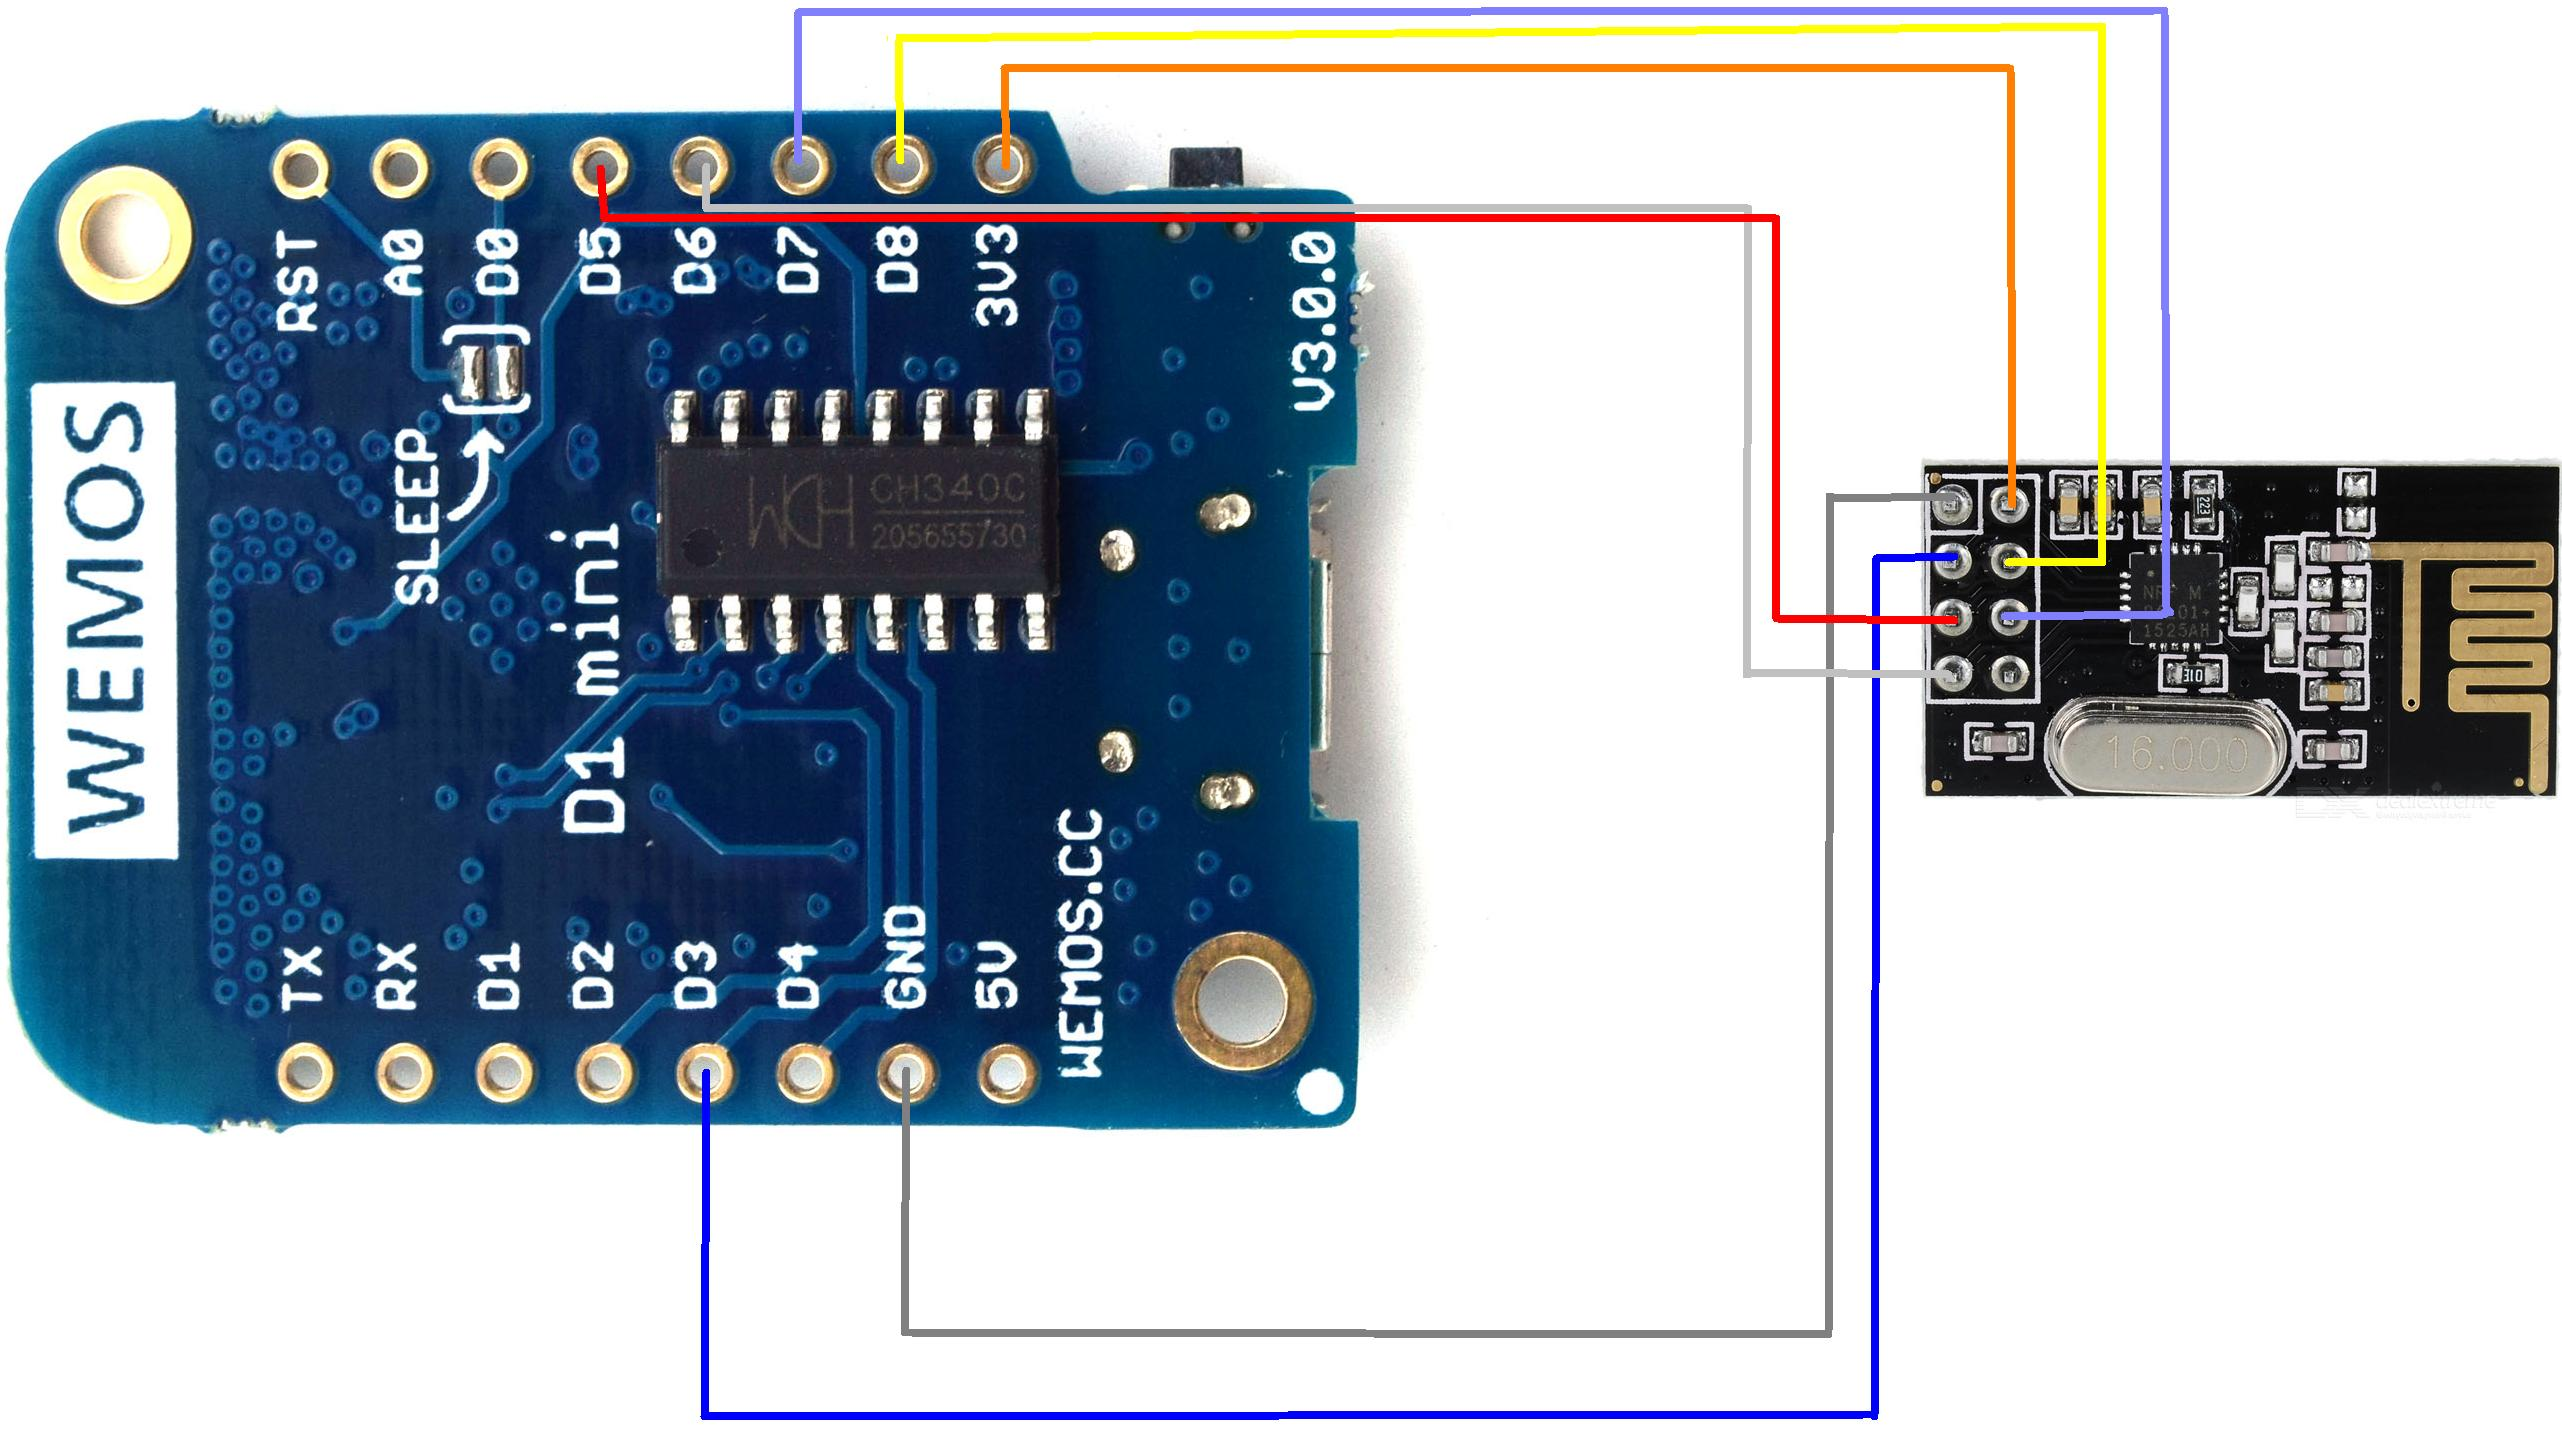
\includegraphics[width=0.35\linewidth]{pinout_coordinator.jpg}
  \caption{Coordinator Pinout}
  \label{fig:pinout_coordinator}
\end{figure}

\paragraph{Configuration}

The configuration for the gateway is shown in~\cref{lst:gateway_config}.

\begin{lstlisting}[language=C++,label=lst:gateway_config,caption="Config Struct for the Gateway"]
struct coordinator_config esp_config = {
  .mqtt_server = "192.168.44.1",
  .mqtt_user = "IoT_client",
  .mqtt_password = "leafy_switch_soup",
  .mqtt_topic_timestamp = "IoT/Time",
  .mqtt_topic_update_interval = "IoT/Interval",
  .mqtt_port = 1883,
  .wifi_ssid = "IoT_17_18",
  .wifi_password = "heavy_cat_radiator",
  .address = 0xF0F0F0F0E1LL,
  .channel = 0,
  .delay = 15,
  .retransmits = 15,
  .auth_key = {0, 0, 0, 0, 0, 0, 0, 0, 0, 0, 0, 0, 0, 0, 0, 0},
  .cepin = 0,
  .cspin = 15,
  .baud_rate = 115200,
  .debug = DEBUG_OFF,
};

\end{lstlisting}

\paragraph{\Gls{mqtt}-Topic Automagic}
The gateway will enforce the mapping between the individual sensors and the respective \gls{mqtt} topics, by constructing the topic from the contents of the LP-RF message (see~\cref{sec:rf_proto}) and augmenting it with the predefined topic parts:
\begin{lstlisting}[]
IoT/Room3/Node5/Sensor2/temperature
\end{lstlisting}
where \lstinline{Iot/Room}, \lstinline{Node} and \lstinline{Sensor} are predefined, and the effective room number (\lstinline{3}), node number (\lstinline{5}), sensor number (\lstinline{2}) and measurement type (\lstinline{temperature}) are defined through the message.

\paragraph{Control messages}

The update frequency of the sensor nodes can be adjusted by sending the desired interval (in seconds) to the topic

\begin{lstlisting}[]
IoT/Interval
\end{lstlisting}

Messages sent to this topic are forwarded by the coordinator to the nodes upon reception of a respective message (since messages \emph{to} the nodes are appended to ACKs).

\paragraph{Known Issues}
\begin{compactitem}
  \item Due to the energy considerations of the protocol (cf.~\cref{sec:rf_proto}), the sensors will adopt a new interval after (worst case) $2*old\_interval$ (where $old_interval$ is the previously set interval, e.g. the default interval), since sensors will only receive data from the coordinator after they send data to the coordinator. 
\end{compactitem}


\subsubsection{Data Broker}
\label{sec:broker}

Following the given conditions by the chosen exercise variant (see~\cref{sec:assignment}), \gls{mqtt} was used as a data broker for all the data from and to the sensor network (cf. \gls{mqtt} mapping in~\cref{sec:gateway}).
For this purpose, \textit{mosquitto}\footnote{\url{https://www.mosquitto.org}} was used, since it is widely known and proven. The following changes were made to the default configuration:

\begin{compactitem}
  \item \textbf{Access authentication} by username and password.
  \item A \textbf{websockets} listener was enabled on port 1884, to make simple web based clients possible, i.e. JavaScript clients (see~\cref{sec:dashboard}).
  \item Secure communication and client authentication through \gls{tls} \emph{with client certificates}.
\end{compactitem}

The configuration is shown in \cref{lst:mosquitto_config}.

\begin{lstlisting}[label=lst:mosquitto_config,caption="Mosquitto configuration"]
  pid_file /var/run/mosquitto.pid

  persistence true
  persistence_location /var/lib/mosquitto/

  log_dest file /var/log/mosquitto/mosquitto.log

  cafile /etc/mosquitto/ca_certificates/ca.pem
  certfile /etc/mosquitto/certs/broker.crt
  keyfile /etc/mosquitto/certs/broker.key

  require_certificate true

  password_file /etc/mosquitto/passwd
  allow_anonymous = false

  port 1883

  listener 1884
  protocol websockets

  cafile /etc/mosquitto/ca_certificates/ca.pem
  certfile /etc/mosquitto/certs/broker.crt
  keyfile /etc/mosquitto/certs/broker.key

  require_certificate true
\end{lstlisting}

The data broker additionally runs a \textit{hostapd} and \textit{dnsmasq} to serve a WiFi \gls{ap} to the gateway device and potential \gls{mqtt} clients subscribing to the sensor data. A systemd script serves as clock source for the sensor network and writes the date and time (sources via ntp) to the \gls{mqtt} topic:

\begin{lstlisting}
  IoT/Time
\end{lstlisting}

\paragraph{Known Issues}
\begin{compactitem}
  \item \textbf{Historic Data} cannot be stored adequately with \gls{mqtt} in general, and shouldn't be stored on the message broker. This responsibility is thus shifted to a/the \gls{mqtt} client, which can then be queried for this data using a different protocol.
\end{compactitem}


\subsubsection{Dashboard}
\label{sec:dashboard}

The dashboard is used to visualize the data from the sensors, being dispatched by the \gls{mqtt} broker (cf.~\cref{sec:broker} and \cref{sec:gateway}). For this purpose, a small website was developed, using the \textit{paho-mqtt.js}\footnote{\url{https://www.eclipse.org/paho/clients/js/}} \gls{mqtt} JavaScript client. This client connects to the broker via websockets, since it runs in the browser and raw tcp sockets are not available for websites/via JavaScript.

For the visualization of the sensor data, the Google Charts library\footnote{\url{https://developers.google.com/chart/}} was used, as a simple way of displaying generic charts in webpages using JavaScript and HTML. Unfortunately, using the library requires Internet access, since content is dynamically loaded from the Google servers.

\paragraph{Known Issues}
\begin{compactitem}
  \item The Google charts library relies on content loaded from the Google servers, which means that the Dashboard can only display charts if the browser running the dashboard has access to the Internet.
  \item Relying on the \gls{mqtt}-broker as data source (cf.~\cref{sec:broker}), the dashboard is restricted to ``live data'' and would need an additional source to query for historic data, e.g. a time-series database as additional \gls{mqtt} client. Retained messages might allow to at least display the last known value.
\end{compactitem}


\subsection{Evaluation}

The setup shown in~\cref{fig:meas_setup} was used to \emph{approximately}\footnote{Since the power consumption of the used test-bed is rapidly fluctuating, the used setup will only approximately show the flowing current.} measure the power consumption of the nodes during typical operation\footnote{1 Emulated Sensor,
wakeup interval = 60sec, no serial print, frequency: 8MHz, without led on atmega board, without led on RTC board}. The circuit was powered with a dedicated power supply, set to 3.3V to avoid destroying the attached RF-module and the FTDI programmer.

\begin{figure}[htb]
  \centering
  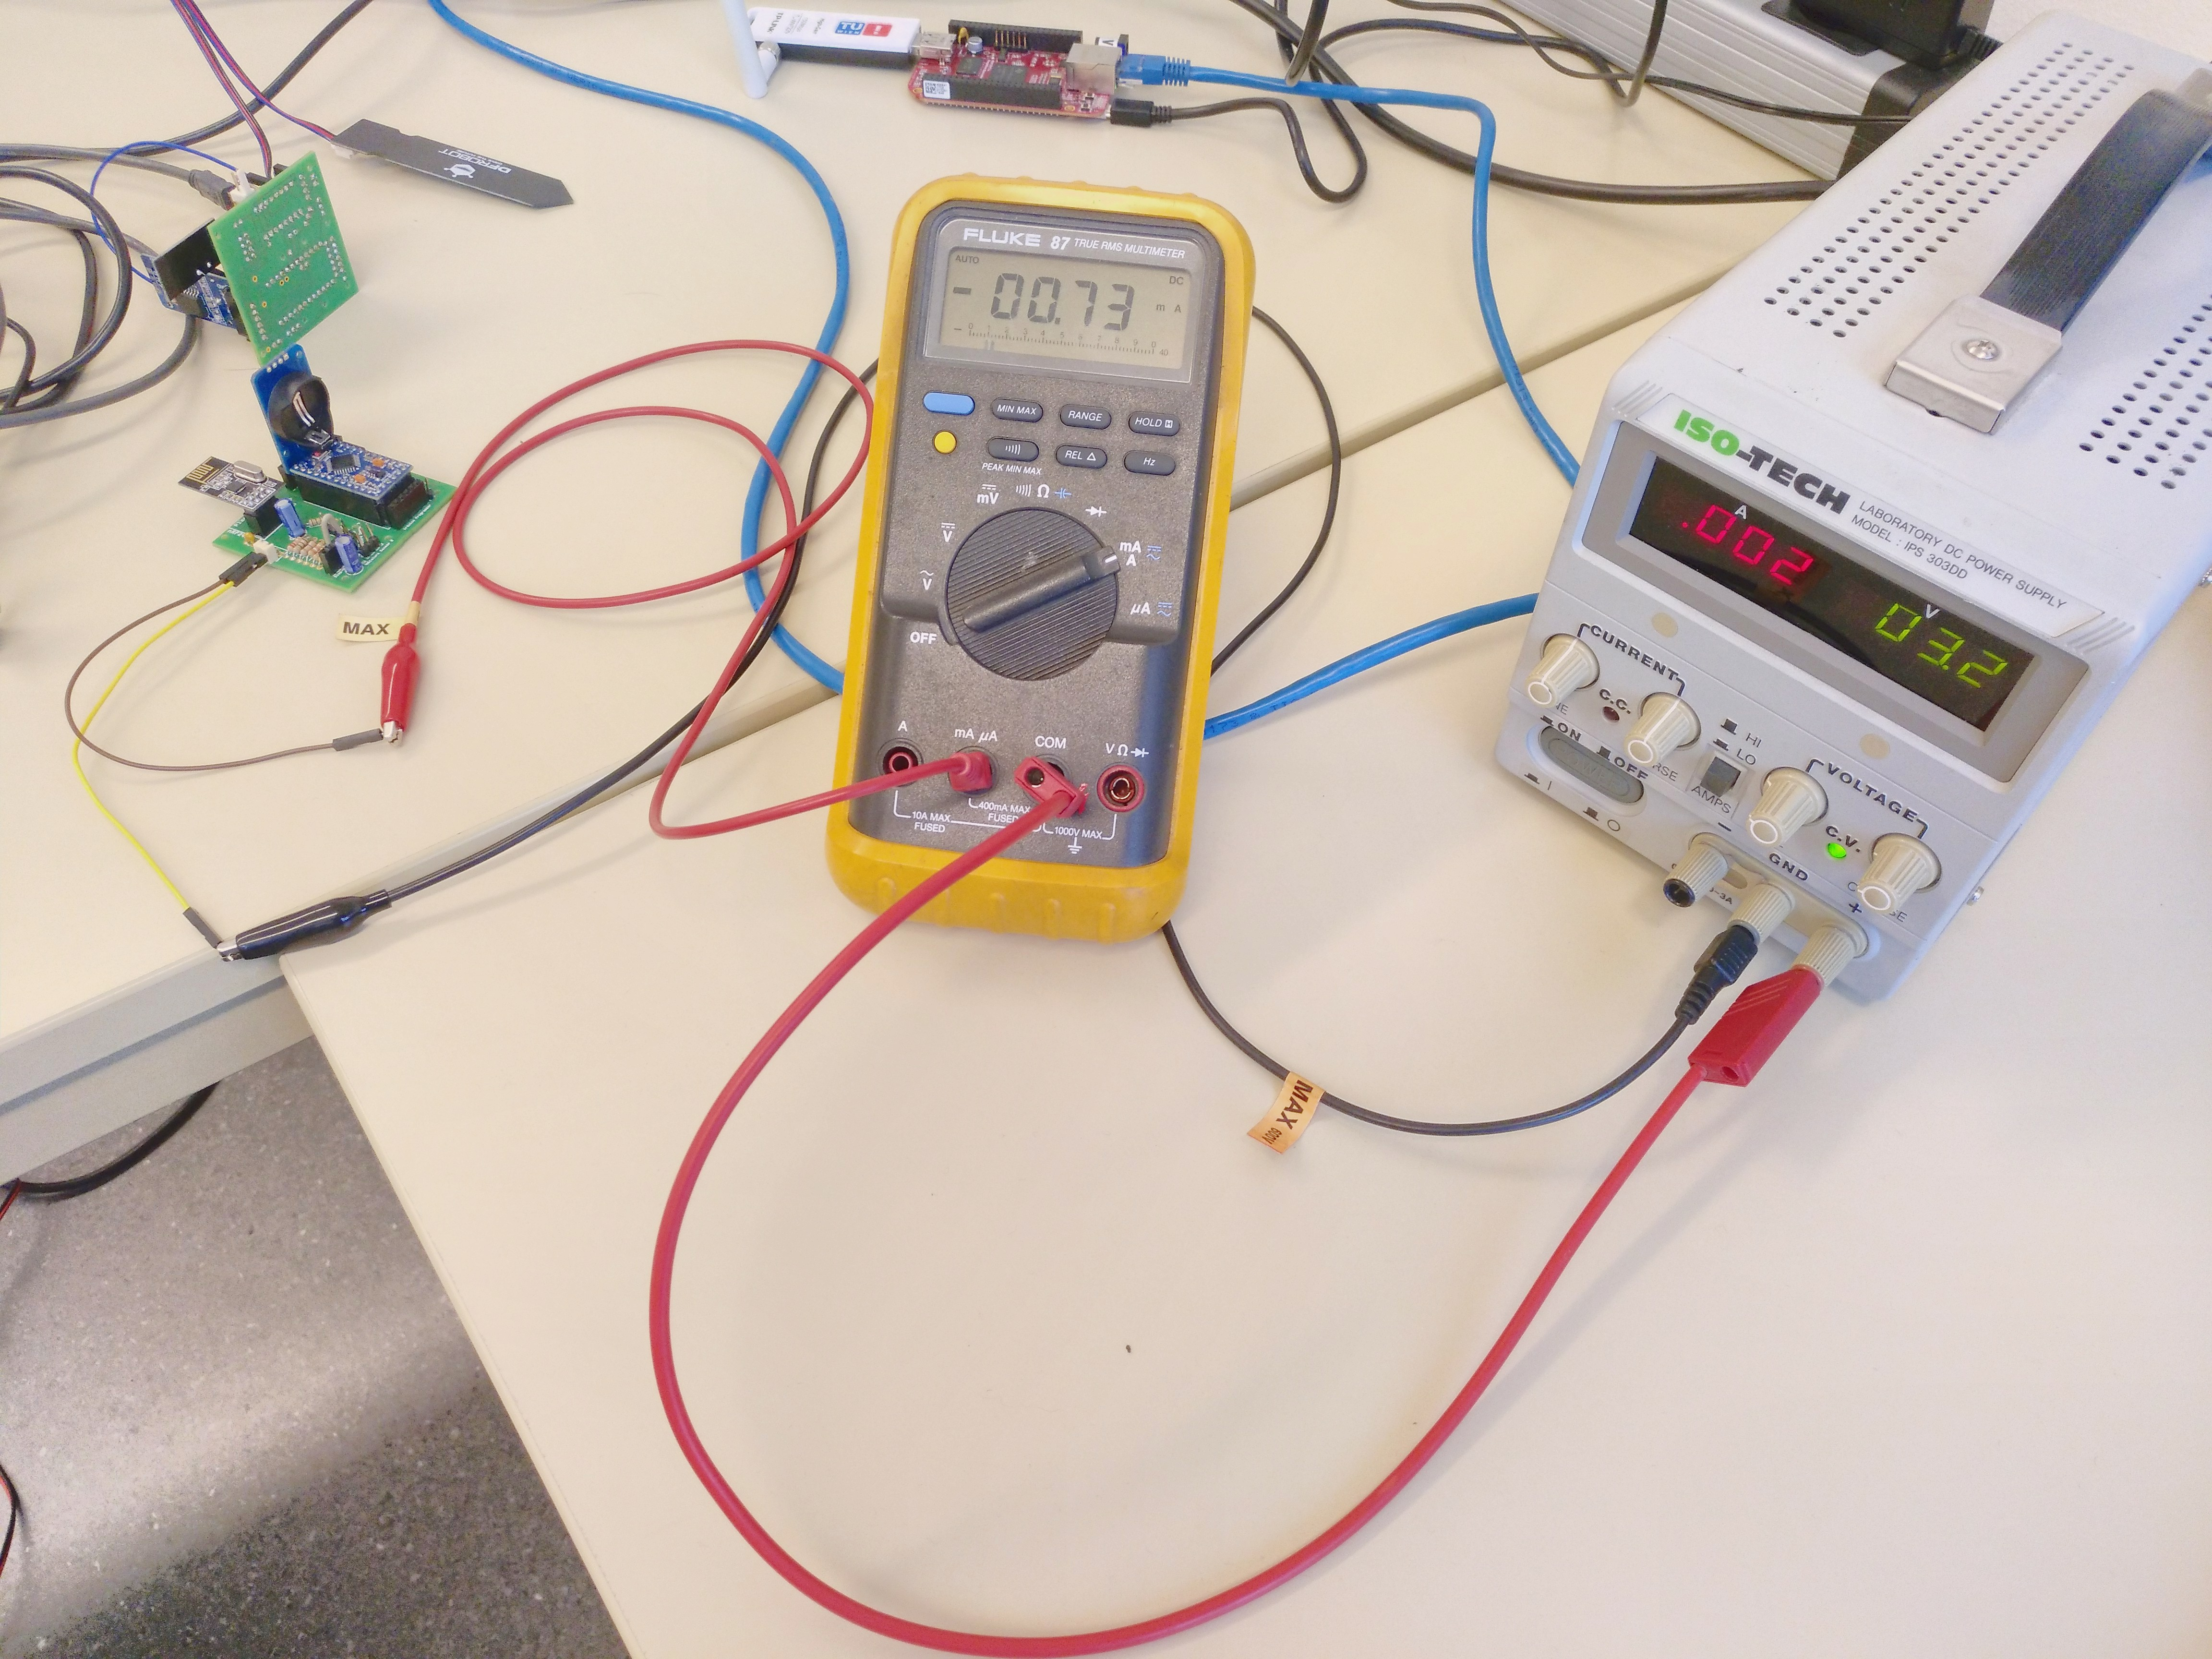
\includegraphics[width=0.55\linewidth]{meas_setup.jpg}
  \caption{Power measurement setup}
  \label{fig:meas_setup}
\end{figure}

Values between \textbf{0.74mA} and \textbf{1.5mA} were measured.


\section{Discussion \& Conclusion}

The assignment could be completed according to the given specification while implementing a few minor additional components. The following concluding remarks might be made:

\paragraph{Underpowered Gateway}

The ESP8266 is slightly underpowered to act as a gateway, which became apparent during development. E.g. smaller key sizes than preferred had to be used for the \gls{tls} client certificates.

\paragraph{Established Solutions}

Established (open) solutions are available for all parts of the LP-RF section of the assignment, from devices (TI MSP430), over operating systems/environments (Contiki, Riot, TinyOS, Thread), to communication protocols (ZigBee, Thread, Sicslowpan, etc.), which offer considerably less power than the components used for the assignment. Similarly, the use of native IPv6 down to the sensor node (e.g. 6LoWPAN, ZigBee, Thread) would have been preferable.

\paragraph{Arduino}

While the Arduino ecosystem brought considerable simplifications and improvements to embedded systems development, the fragmented and frayed library ecosystem of voluntary contributions with varying degrees of capabilities results in unforeseeable bug hunting sessions, since the quality and active maintenance of libraries is not known beforehand. While great for hobbyists and proof of concept implementations, it is considered less suited for the production in the scope of commercial products or for more elaborate scientific work.

%!TEX root = ../proj_docu.tex

\singlespacing

{\small
\setglossarystyle{index}
\printglossary[type=\acronymtype]
%\vspace{-2\topsep}
\printglossary
}

\setlength\bibitemsep{0pt}
\vspace{-2\topsep}
\printbibliography[heading=bibintoc]
%%!TEX root = ../proj_docu.tex

\singlespacing

{\small
\setglossarystyle{index}
\printglossary[type=\acronymtype]
%\vspace{-2\topsep}
\printglossary
}

\setlength\bibitemsep{0pt}
\vspace{-2\topsep}
\printbibliography[heading=bibintoc]

% %!TEX root = ../proj_docu.tex

\appendix
\pagenumbering{Alph}



\end{document}